\documentclass[a4paper,12pt,hidelinks]{report}
\usepackage{graphicx}
\usepackage[parfill]{parskip}
\usepackage[backend=bibtex,style=ieee]{biblatex}
\usepackage{fancyhdr}
\usepackage[top=3cm,bottom=3cm,left=3cm,right=3cm,headheight=15pt]{geometry}
\usepackage{gentium}
\usepackage{titlesec}
\usepackage{placeins}
\usepackage{caption}
\usepackage{subcaption}
\usepackage{textcomp}
\usepackage[UKenglish]{isodate}
\usepackage{blindtext}
\usepackage{pdflscape}
\usepackage{tabularx}
\usepackage{longtable}
\usepackage{pdfpages}

\usepackage[pdftex,pdfauthor={Dale Mark Peters (Student Number 120062861)},pdftitle={SE31520 Assignment Documentation | Aberystwyth University},pdfcreator={pdflatex}]{hyperref}

\title{SE31520 Assignment Report}
\author{Dale Mark Peters}
\graphicspath{{/home/dale/university/se31520/assignment/report/images/}}

\bibliography{bibliography}
\captionsetup{width=0.8\textwidth,font={small}}

\titleformat
{\chapter}
[block]
{\bfseries\huge}
{\thechapter}
{3ex}
{}
[]

\pagestyle{fancy}
\fancyhf{}
\lhead[LO]{\leftmark}
\rhead[RE]{\rightmark}
\cfoot{\thepage}
\begin{document}

\maketitle

\tableofcontents
\chapter{Introduction}
    This document is written to accompany the software I have written for the SE31520 (Developing Internet Based Applications) 2015-2016 assignment. In this
    document, I will describe the architecture and justify the design of my web application and RESTful APIs developed, and will then go on
    to explain the testing strategy used for my applications and give the results of the tests. Finally, I will give an evaluation of how well the requirements
    were met and how well I have done in the assignment.

    In this assignment, I was tasked with the design and implementation of a web application (My Alcohol Free Wines - from now on called MAF) that allows users to find the cheapest prices
    for the non-alcoholic wines they wish to buy. This had to be done by comparing the prices of one identical wine from two different suppliers and displaying the
    cheapest one in the MAF wines listing page. From the wines listings page, the idea was that they can then place their desired wines into their basket and place
    an order, where an `order' consists of sending the details of the purchase and the customer details to the relevant supplier via a RESTful request.

    My system was developed and tested on a machine running Ubuntu 15.04, in Google Chrome and Mozilla Firefox. The MAF application can be run using \texttt{rails s} from
    the `my-alcohol-free-wines' directory and the service can be run using \texttt{python ./app.py} from the `service' directory.

\chapter{Design/Architecture}
    \section{Use Case Diagram}
    \begin{center}
        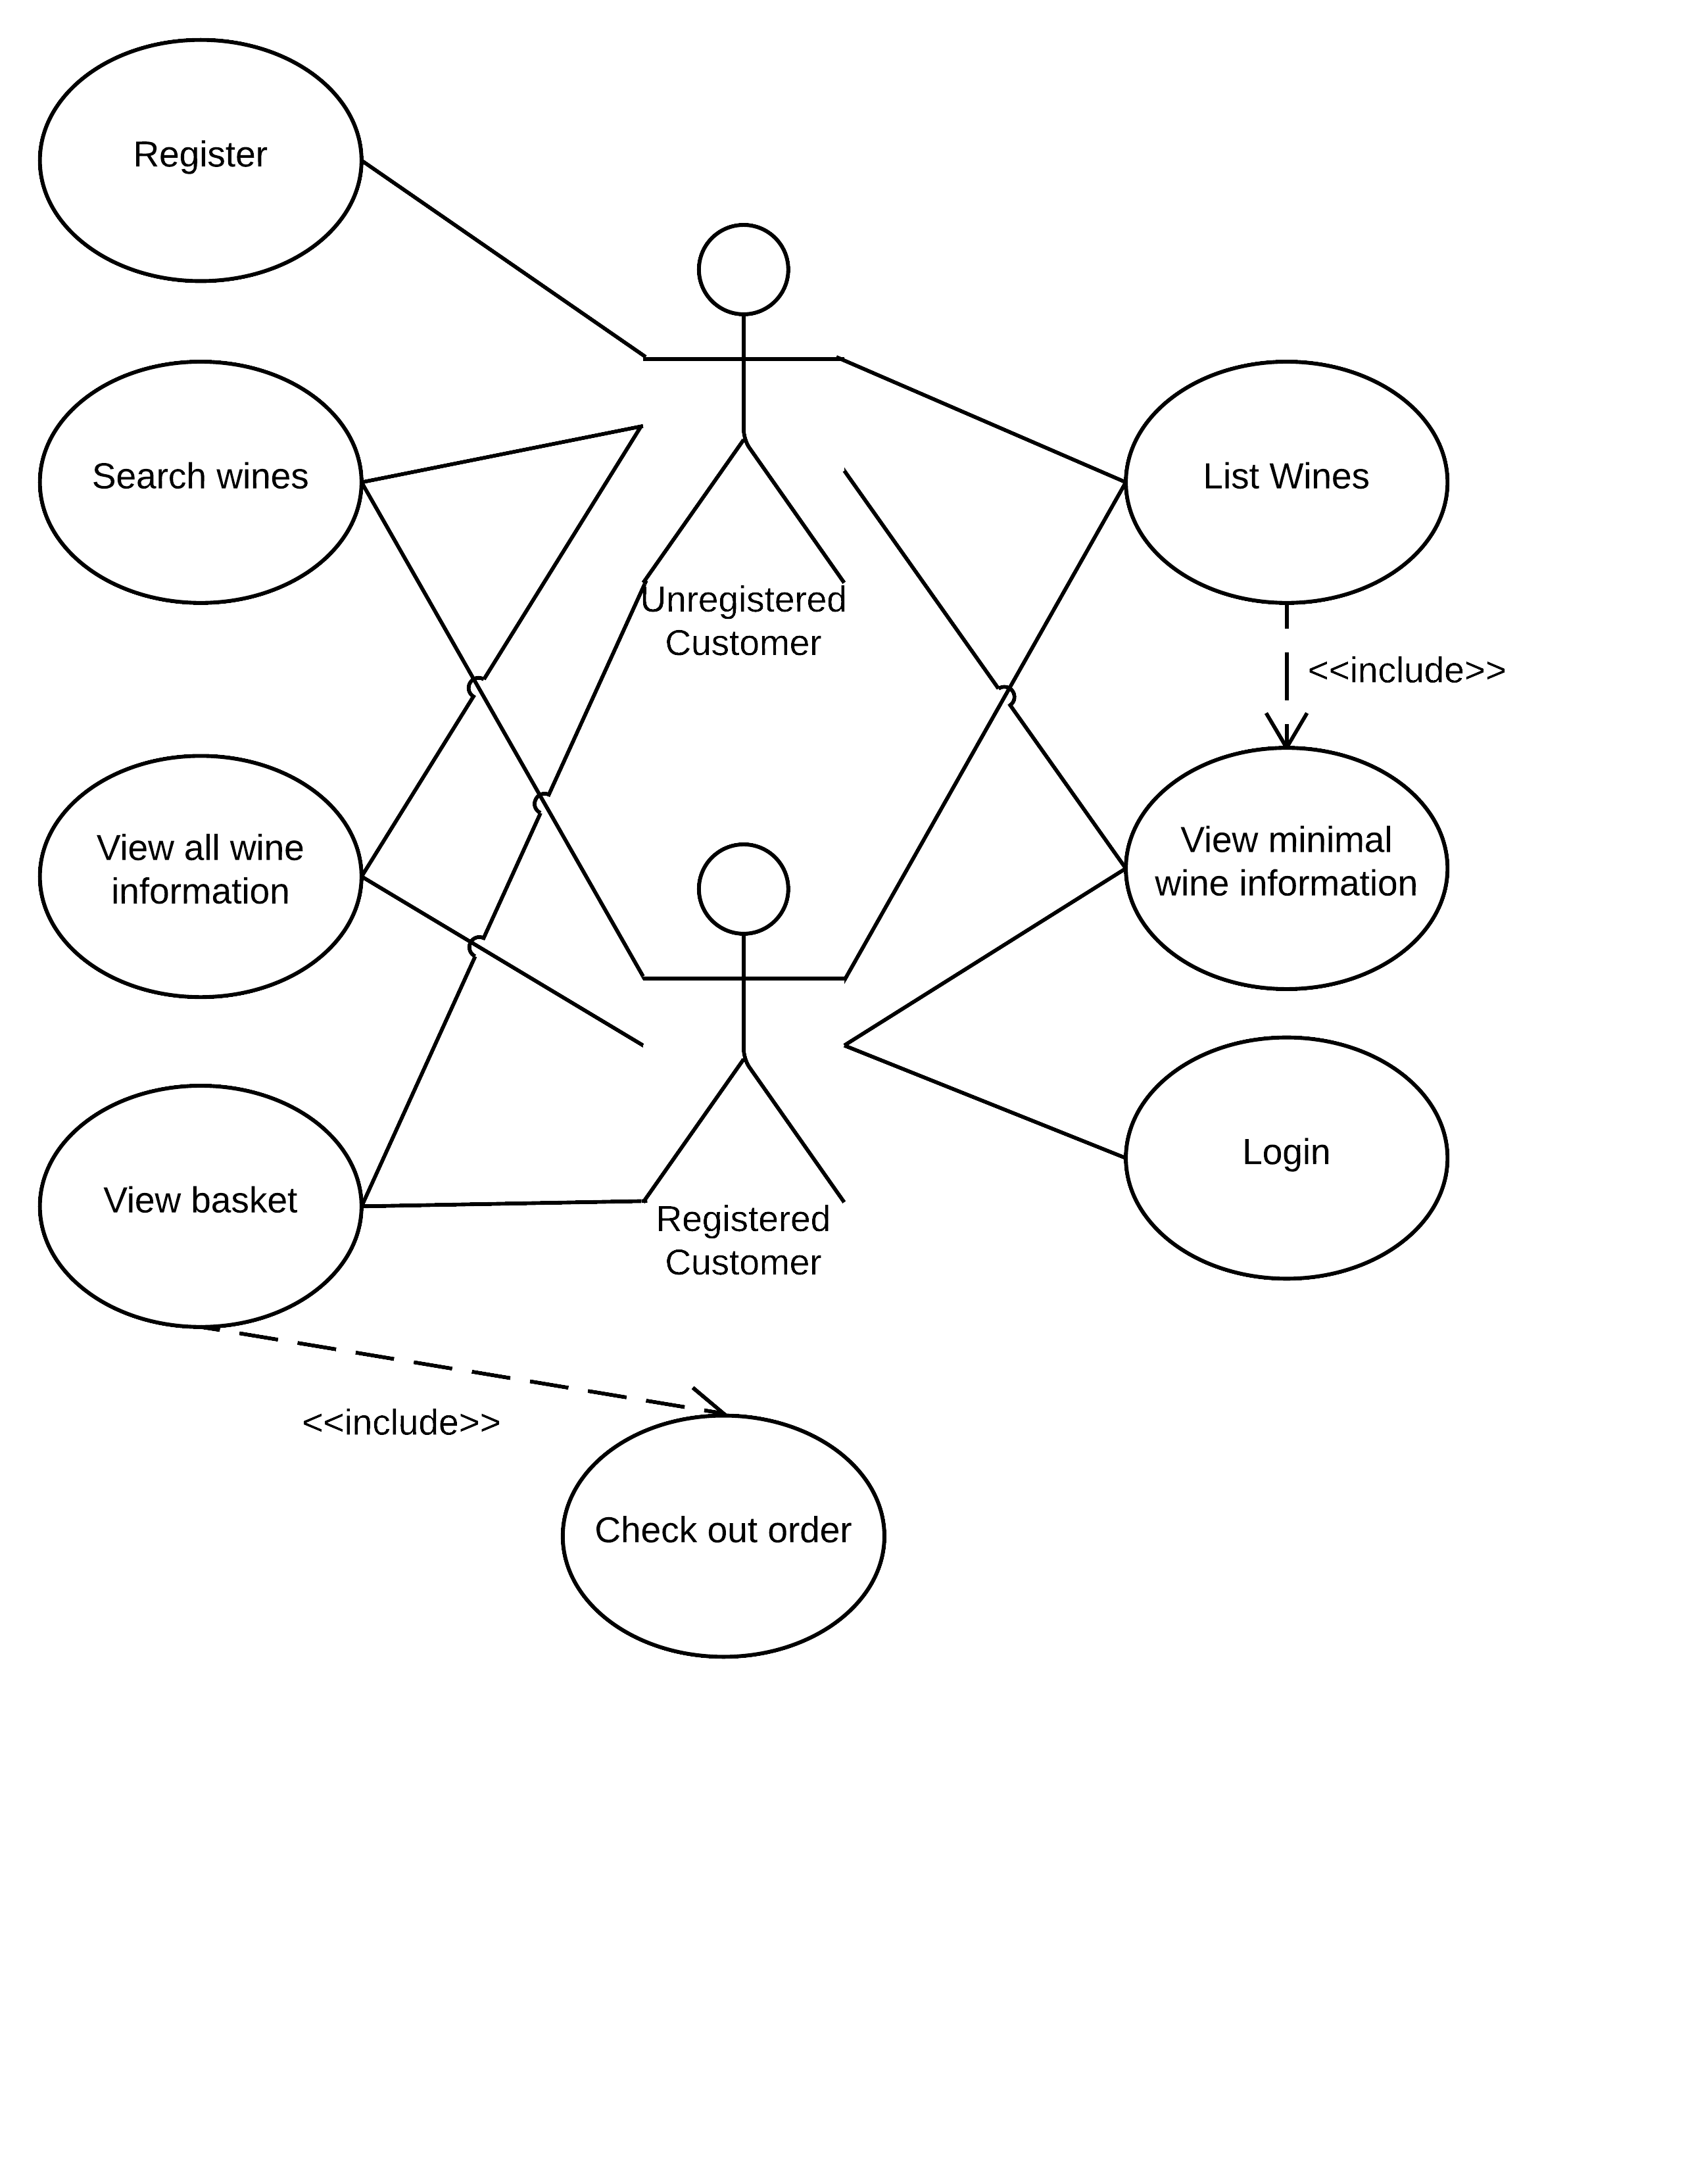
\includegraphics[scale=0.60]{use-case-diagram.png}
    \end{center}

    \section{Architecture Diagram}
    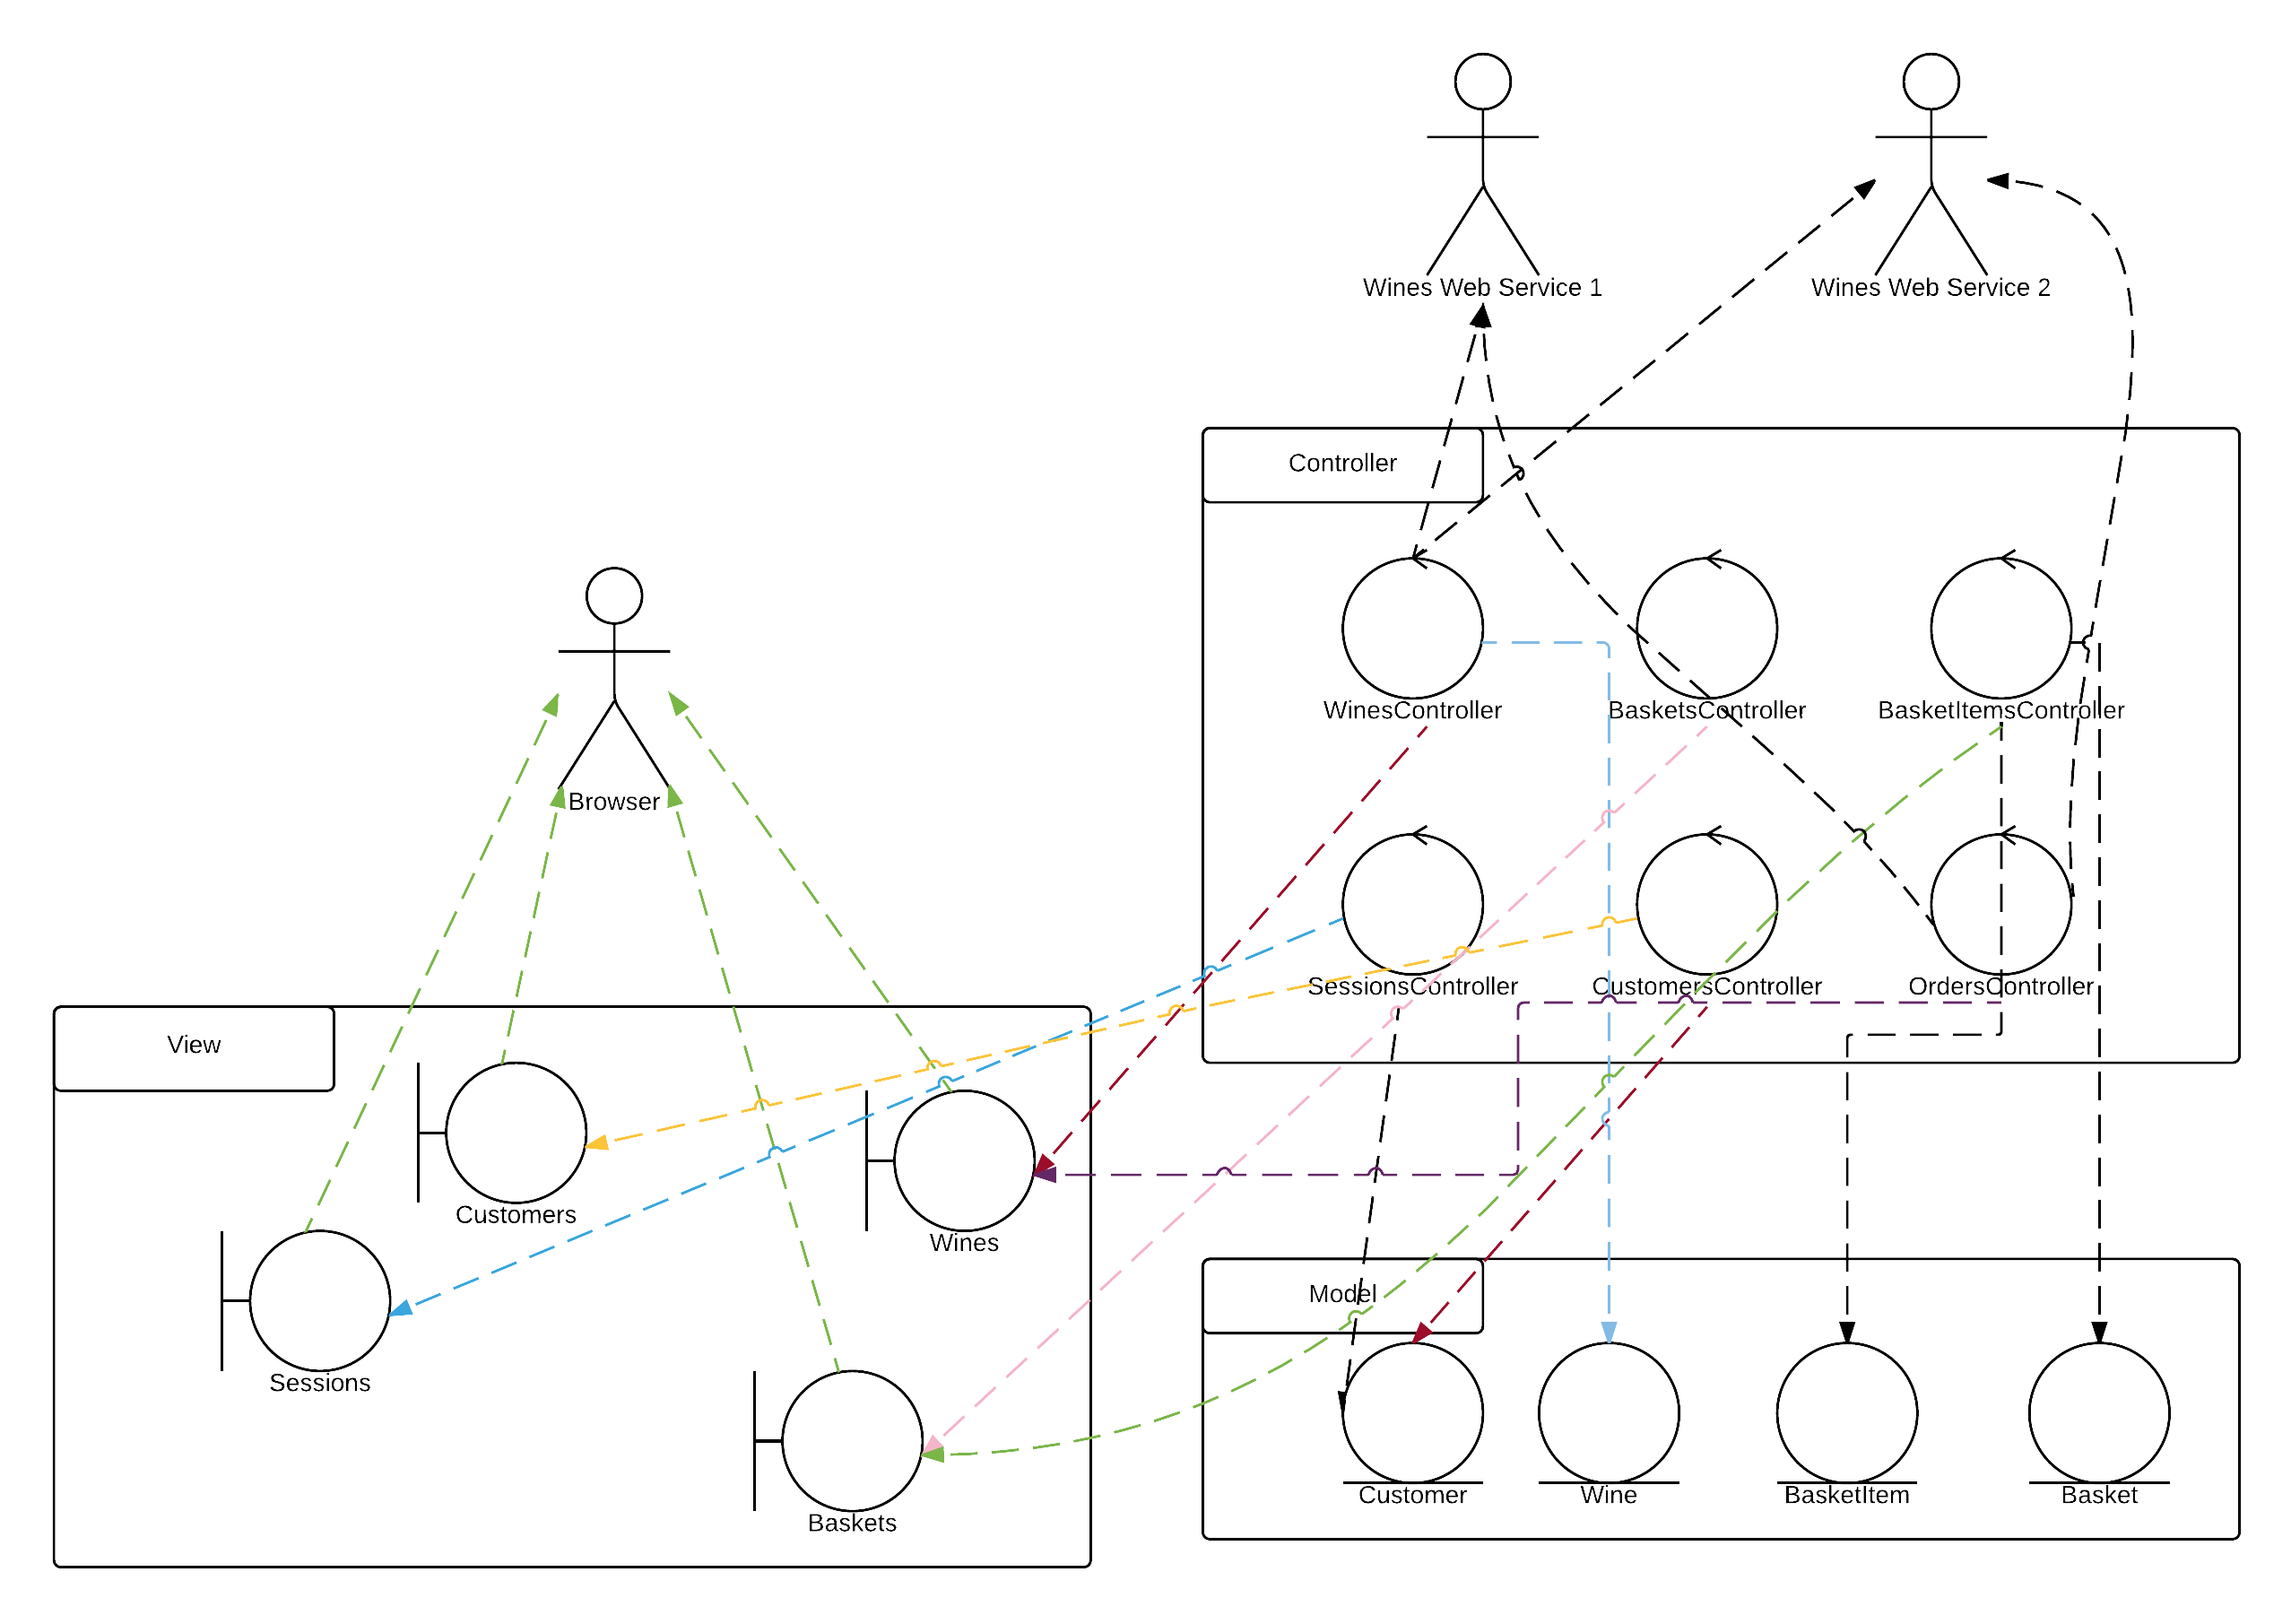
\includegraphics[width=\textwidth]{architecture-diagram.png}
    \section{My Alcohol Free Wines}

    \subsection{Data Models (Classes)}
    From the specification of the assignment and the system that needs to be implemented, some of the models that needed to be considered were clear.
    These are detailed in this section.
    
    \subsubsection{Wine}
    The most important of the models to be implemented in the application was the Wine model, which represents a product MAF sells. Most of its attributes
    can be represented by a string as they are textual attributes of the product. Both descriptions, the bottle size, the origin country, the bottle size, the supplier
    and the grape types can all be represented textually, so I chose a string representation for these.
    
    The price field, however, could be a decimalised amount, so I chose a float representation for these. Also to be stored was the suitability for vegetarians, which 
    is a binary concept, so I chose a boolean representation for this. 
    
    A field I added but is not mentioned in the specification is some form of unique identifier to distinguish the same product from
    two difference suppliers. I therefore added a barcode field so that a wine from a particular supplier could be compared to the same wine from the other
    supplier which might have different information. I chose a string representation for this to cover cases where it might begin with a 0.

    \subsubsection{Customer}
    I have implemented a customer model to represent the customers who might be purchasing from MAF\@. All the information to be stored about customers was
    to be stored in the form of a string, as all the information to be stored about customers is textual. Another field I had to add to the database for this
    model but wasn't specified in the specification was the password digest field, which is required by the Ruby bcrypt gem to hash the customer passwords.
    It also makes sense that each customer holds a basket, so I added this field to the database to hold the foreign key reference to the user's basket id,
    but I didn't get round to completing the implementation for this.

    \subsubsection{BasketItem}
    It is clear from the specification that the basket in the MAF application could potentially hold several Wine items if the customer wants to add
    several wines to their basket. It is therefore necessary to have a model that links these two models up. By having this in a separate table, I
    can have as many items as desired in the table without having to have a separate column for each product in the basket. In the way I have designed it,
    the database table just needs two foreign key references - one specifying which wine the item of the basket represents, and the other representing the
    basket it belongs to. Another field is the quantity, which contains the quantity of that particular item there are in the basket.

    \subsubsection{Basket}
    The specification states that customers should be able to add wine items to their basket, and so it is necessary for a basket to represent
    a collection of products the customer wants to buy. There isn't really much information about this in the specification, so in the database,
    my implementation just has an ID and no other attributes.

    \subsection{Controllers}
    With Ruby on Rails being a MVC framework, it was important to define several controllers for use in the application.

    Each of the models described in the previous section have an associated controller so that requests between the browser and the MAF
    application are handled appropriately. Each of these controllers have a method defined for each of the request types (one for each of GET, POST, 
    PUT/PATCH and DELETE), as these were generated automatically when I ran the \texttt{rails generate scaffold} command. In hindsight, I could have
    only generated the necessary methods to meet the requirements.

    As an example, for the Customers controller, I could have just generated methods for creating a new customer, as there is no requirement 
    for functionality to edit or delete a customer's details or show the details for a particular customer. 
    
    The Wines controller is also responsible for getting the wines from the supplier service, which is done by getting the response and parses the
    JSON, converting them to objects to be stored in the database if it is not already in there. If I had the time to implement the second one,
    I would have done this by comparing each barcode to the ones already in there and only adding it to the database if it is cheaper.
    
    In addition to the controllers for the models, I also had to implement an Orders controller and a Sessions controller. These are responsible
    for the sending of the order to the wine supplier API and the logging in and out of the customers respectively. The reason for creating the 
    orders controller was that it didn't really make sense to put it in any of the other classes, as it involves something completely different.
    I could have implemented a model for the Orders so as to improve the separation of concerns, and just had the Orders controller communicate
    with the basket page (where the user checks out) and the model. This controller only has a method for creating the order, which is
    also the one that sends the order to the supplier, as this is the only thing that was necessary to implement. The sessions controller also
    has a limited number of functions, as it is only necessary for a session to be created or destroyed - it doesn't make any sense to allow a session
    to be edited or shown.

    \section{RESTful Supplier Web Service}
    \subsection{Programming Language}
    I decided to implement the supplier RESTful API in Python, making use of the Flask framework \cite{flask-framework}, as I have a lot of experience in
    Python and it is a language I feel comfortable using. It was also possible to implement the service with a very small amount of code.
    I'd never used the Flask framework before or created a RESTful API, but it allows the simple set up of routes with methods. Included in
    my submission is the code for the service, but it also includes the necessary files for Flask to run. These are contained in the `flask' directory.
    The only code I wrote for the web service was that in service/app.py.

    \subsection{Routes}
    In comparison to the MAF design, the design of the web service I have implemented is very simple. Since the requirement of the services was
    to just provide an interface for receiving orders from the MAF website and providing a list of wines to the MAF application to list on the website,
    I only needed to implement support for GET requests for wines and POST requests for orders, so I defined routes in the service code to handle these.
    I also thought it would be useful to implement GET support for the orders for testing purposes, so I defined this route too. The service runs on
    the local machine on port 5000, so the POST orders route is \url{http://localhost:5000/orders/} and the GET wines route is \url{http://localhost:5000/wines/}.

    \subsection{Storage of the Data}
    Because of the simplicity of this application, I didn't feel the need to implement Order and Wine models like with the MAF application. Instead,
    I just store a list of the wines and orders in a Python list of dictionaries, each containing the data about the wines and the orders. These are stored
    in memory in the current implementation, but if I was to improve this, I would store these in a database or a file instead, which would separate the
    concerns.
    
    \subsection{Communication of Data}
    For the communication of the information, I chose a JSON representation, since Python has functions available to convert a Python dictionary into
    a JSON object easily, and Ruby also offers functionality to convert hashes into JSON objects. JSON also has the advantage that no particular
    schema is required for the information and less text is needed to represent the entities than in, say, XML, for example.

\chapter{Third Party Libraries/Code/Assets}
    Whilst doing this assignment, in order to reduce the amount of time it took me to develop the application, I used several third party
    Ruby on Rails gems in addition to the ones that are in a default Rails project. These are from \cite{gems} and are listed in the Gemfile, 
    but are also as follows:
    \begin{itemize}
        \item \textbf{rest-client}: Used for the sending of requests from the MAF application to the two RESTful APIs.
        \item \textbf{bcrypt}: Used for the encryption of the customer's user name and password.
        \item \textbf{will\_paginate-bootstrap}: Used for the Bootstrap-style pagination of the wines in the wines listing page.
        \item \textbf{activerecord-session\_store}: Used to store sessions in a database.
        \item \textbf{will\_paginate}: Used for pagination of the wines in the wines listings page
        \item Various gems for testing, including cucumber-rails, database\_cleaner, factory\_girl, rspec-rails, selenium-webdriver and capybara.
    \end{itemize}

    For the styling of the website, I used Bootstrap CSS, which is contained in the files with names beginning with `bootstrap' in the app/assets/stylesheets
    directory. This was obtained from \cite{bootstrap}.

    The image for the wine was obtained from \cite{wine-image}.

    For the logging in/out functionality, I followed an online tutorial and so my code is based on the example code snippets given in the tutorial (\cite{online-ruby-book}) and
    for the basket functionality, I followed the guidance of the recommended reading for the module, so my code is based on examples given in that book (\cite{agile-web-dev}).
    I have put comments in my code to acknowledge where my code is based on examples from other sources.

\chapter{Testing}
    \section{Discussion of System Tests}
    For the testing part of this assignment, I first of all made a 
    test table (found in the appendices of this document). In this,
    I took each of the requirements given in the specification and identified the key parts of each of them and put it into a
    table. Some of the requirements have multiple tests to ensure that things don't happen when they aren't meant to, such as results
    being displayed in the search results when the query doesn't actually match anything. I have commented on each of these
    in the test table in the Comments column. 
    
    Most of the test failures were down, in part, to time constraints I had for completing
    the assignment. Because I didn't have time to implement the second service, for example, the test for searching for wines
    from both suppliers failed.

    Another one that failed was the sending of the order information to the web service. This is because I was unable to get
    the basket details from the checkout page to send off to the web service. Customers were also unable to checkout without
    logging in first.

    \section{Cucumber Testing}
    The testing of the system then continued with me writing Cucumber tests for acceptance tests based on the requirements.
    I wrote one of these for the search feature, one for the listing all the wines search and one for the `Show' page for
    the wines. The first step for writing these tests was to write out some feature files, which contains human-readable text defining
    what data we have, what action is going to happen, and what result is expected from doing the test. There is then a step\_definitions
    file which tells the Cucumber gem what to do when it comes to a certain phrase in the feature file. For my tests, these are contained
    in the step\_definitions/wine\_steps.rb file.

    The first two of these tests passed all the defined steps, which means that the software client could have confidence that these
    requirements are implemented successfully and that the functionality works. The third of these tests failed due to the fact that I couldn't
    work out how to get the Capybara gem to click on an image automatically. I have read in documentation that it is possible to
    search for a particular element in the XML tree by using traversal, but I couldn't work out how to use this.

\chapter{Self Evaluation}
    \section{Screencast}
    Unfortunately, I was unable to do a screencast of my application running due to the fact that I couldn't get a screencasting
    software package to work on my machine. I therefore had to provide a series of screenshots in a document (screenshots.pdf) to provide evidence
    that my application and service run. I hope that the screenshots provide sufficient evidence for this. My screenshots aren't able
    to show a second implementation working as I didn't have time to implement the second one. I would award myself \textbf{5/10} for this.

    \section{Design}
    When I first started this assignment, I struggled to remember some of the concepts of OO design as it has been over a year since
    I did any. For the design, I feel that I have done well in representing the underlying models that represent the real world objects and
    giving rationale for the design. Where there are room for improvements, I have detailed this in my Design section. I feel that I could 
    have added something to explain how my design complies with the design
    constraints. I have learned how to apply an MVC design pattern for the first time in doing this assignment. I would award myself
    \textbf{10/20} for this section.

    \section{MAF Implementation}
    Overall, I am quite pleased with how well my MAF application works, as the application runs well and I used the features of Rails
    well to generate the scaffolds. I also made effective use of migrations in order to make any necessary changes to my models
    as I developed the application. I do feel that my code is well commented and the code is of a good, readable quality. However, the separation
    of concerns could have been done better, in accordance with the MVC design pattern. I also believe that I could have developed the controllers
    with fewer methods to restrict the access to the entities such as customers and wines. I would award myself \textbf{15/25} for this part of the assignment.

    \section{Supplier Implementations}
    I personally found that the implementation of my service was very easy to do with the Flask framework, but my code quality suffered a little
    by the fact that I kept the list of wines in the same file and the orders in memory. I could have improved this by putting them in 
    a separate file. I would give myself \textbf{8/15} for this.

    \section{Testing}
    My testing table included in the appendix of this report is, in my opinion, very thorough and I feel as though I covered all
    the requirements given in the specification well. I have commented on each of the tests and said where potential
    design flaws are in terms of usability and in terms of requirements. In doing the testing for this assignment, I learned how to
    write Cucumber tests to test the behaviour of a Rails application the importance of them. My downfall in this section was not having
    the time to write any unit tests, so all the ones included in this submission are automatically generated by the Rails framework.
    I would therefore give myself \textbf{8/15} for this.
    
    \section{Flair}
    I didn't really add much to the application or the web service in addition to the requirements. One thing I did do was allow the
    customer to remove items from their basket, and allow them to add wines to their basket from the Wines listings page. The use of the
    Bootstrap stylesheet also means that my app is responsive to smaller browser window sizes. I would therefore give myself \textbf{3/10}
    for this.

\printbibliography

\titleformat
{\chapter}
[block]
{\bfseries\huge}
{Appendix \thechapter:}
{3ex}
{}
[]
\appendix
\chapter{System Test Table}
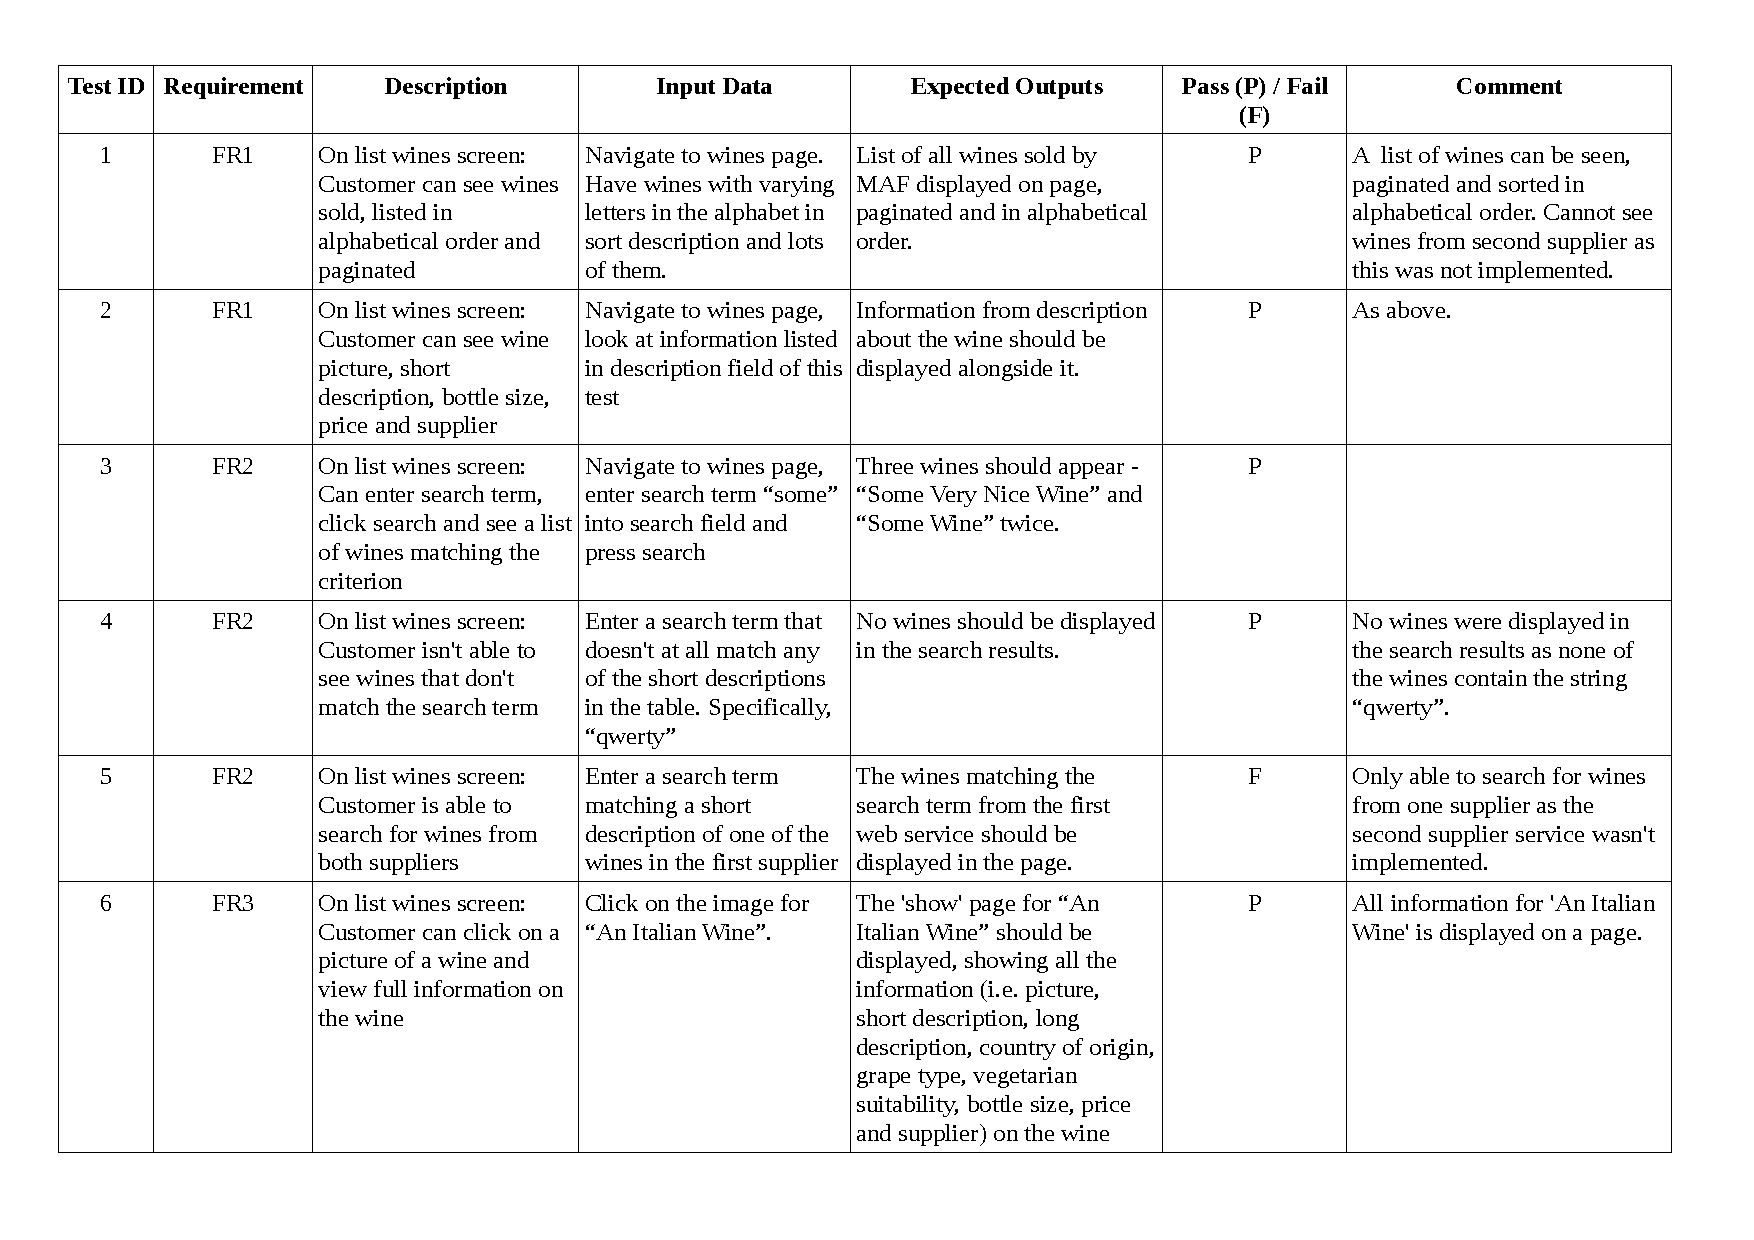
\includepdf[pages={-}, angle=90]{images/test-table.pdf}

\end{document}
